% Short submission (three pages at most), drafted by Claude for Salah's revision.
% Interpretations: in the results they open with an italic "Interpretation." run-in,
% and the Discussion and Conclusion are interpretive by their titles. Salah confirms,
% rewrites or removes each of them. Every reference was checked at its source on 2026-11-21.
% The extended version, with every detail, is do-autointerp-scorers-agree-extended.tex.
% Compile with: tectonic do-autointerp-scorers-agree.tex
\documentclass[10pt]{article}
\usepackage[utf8]{inputenc}
\usepackage[T1]{fontenc}
\usepackage[english]{babel}
\usepackage[a4paper, margin=1.8cm, top=1.5cm, bottom=1.6cm]{geometry}
\usepackage{amsmath}
\usepackage{graphicx}
\usepackage{booktabs}
\usepackage{xcolor}
\usepackage{enumitem}
\usepackage[font=footnotesize, labelfont=bf, skip=4pt]{caption}
\usepackage{hyperref}
\hypersetup{colorlinks=true, urlcolor=blue, linkcolor=blue, breaklinks=true}
\graphicspath{{../figures/}}
\tolerance=2000
\setlength{\emergencystretch}{3em}
\setlength{\parindent}{0pt}
\setlength{\parskip}{3.5pt}
\setlength{\footnotesep}{6pt}
\makeatletter
\renewcommand\section{\@startsection{section}{1}{\z@}{-1.8ex}{0.8ex}{\normalfont\large\bfseries}}
\renewcommand\subsection{\@startsection{subsection}{2}{\z@}{-1.3ex}{0.4ex}{\normalfont\normalsize\bfseries}}
\renewcommand\@makefntext[1]{\noindent\footnotesize\textbf{\@thefnmark.}\ #1}
\makeatother
\newcommand{\bibentree}[1]{\par\noindent\hangindent=1.2em\hangafter=1 #1\par}

\begin{document}

\begin{center}
{\Large\bfseries Do autointerp scorers agree?}\\[3pt]
{\large Five LLM scorers, one SAE, and a placebo control}\\[5pt]
{\small Salah Chadli $\cdot$ Mechanistic Interpretability Hackathon 5: Autointerp, November 2026}\\[1pt]
{\small Code and data: \url{https://github.com/chadlis/scorer-agreement}}
\end{center}

\section{Question and motivation}

A \emph{sparse autoencoder} (SAE) splits the activations of a language model into many
\emph{features}, each meant to stand for one idea, and an LLM writes a short
\emph{explanation} of each. In \emph{detection} scoring (Paulo et al., 2024), a second
LLM, the \emph{scorer}, reads the explanation and one text, and answers 1 if it predicts
that the feature fires on the text. The share of right answers is the score of the
explanation.

The score thus depends on two things: the explanation, which one wants to measure, and
the scorer, which is a choice of the pipeline. Van der Ben et al.\ (2026) show that
pipeline choices move autointerp scores a great deal. They keep one scorer fixed, Gemini
Flash, and name the variation of the scorer as an axis they did not
study\footnote{``All scoring uses Gemini Flash as the fixed scorer'' (section 2), and
``scorer variation and layer-dependence are additional axes of instability we did not
study'' (section 5). Van der Ben et al.\ 2026.}. Chen (2026), for his part, shows that
a rule that never reads the explanation can beat LLM scorers on stored scoring
data\footnote{On the stored runs of Neuronpedia for GPT-2 small, a rule that answers
``yes'' when the central token of the excerpt is marked reaches a balanced accuracy of
0.979, against 0.838 for the stored LLM scorers. Chen 2026, abstract.}, and he
recommends reporting every score next to an explanation-free baseline.

Scorers have been compared before. Paulo et al.\ already compare three scorers on the
same explanations, through their median scores\footnote{Claude Sonnet 3.5, Llama 70B and
Llama 8B, in appendix F.7 (table A9) of Paulo et al.\ 2024.}, and Chen compares
simulators on identical inputs with original and shuffled explanations. To my knowledge
(searches of 17 and 21 November 2026), no study measures, for several detection scorers,
their agreement text by text, the gain that each draws over an explanation-free control,
and whether their disagreements change which explanation is preferred. I therefore ask:

\begin{center}
\begin{minipage}{0.86\linewidth}
\emph{With texts and explanations held fixed, do scorers differ in their judgments, and in
the gain that the explanation brings them over an unrelated explanation (a placebo)?}
\end{minipage}
\end{center}

This study makes three contributions.
\begin{enumerate}[leftmargin=1.4em, itemsep=2pt, topsep=2pt]
\item It measures how often five detection scorers disagree on the same text, and not
only whether their mean scores agree: two scorers answer differently on 7 to 13\% of the
texts.
\item It measures, for each scorer and on exactly the same texts, the gain that the
explanation brings over a placebo, so that the gains can be compared pair by pair: four
scorers gain about the same, and Opus about 3 points more.
\item In an exploratory analysis decided after the results, it asks whether these
disagreements change which of two explanations of a feature a researcher would keep: two
scorers pick opposite explanations on 13 to 27\% of the features.
\end{enumerate}

\section{Design}

\begin{figure}[h]
\centering
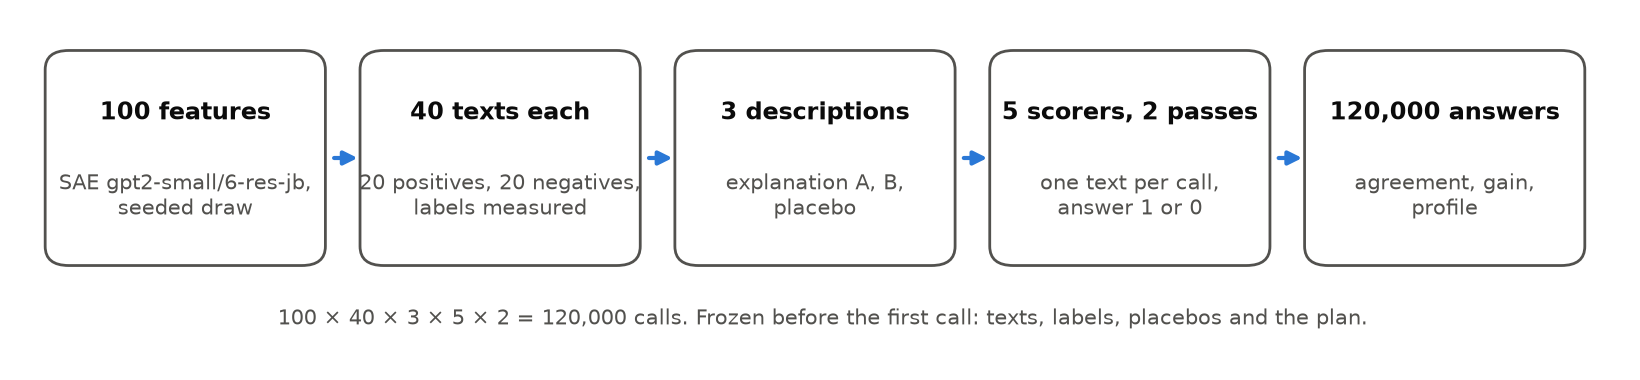
\includegraphics[width=0.78\linewidth]{fig0_design.png}
\caption{The design. Texts, labels, placebos and the analysis plan were frozen in git
before the first scorer call (tag \texttt{plan-frozen}).}
\end{figure}

\textbf{Features.} I drew 100 features of the SAE \texttt{gpt2-small/6-res-jb}
(Neuronpedia), with a published seed, among those that fire on 0.001\% to 1\% of tokens
and have two original explanations: A, written by gpt-3.5-turbo, and B, by
gpt-4o-mini\footnote{Of the first 114 features examined, 5 failed the frequency filter,
8 failed a gate (their strongest stored window must still fire when sent alone), and one
kept too few positives after recomputation and was replaced by the next feature of the
draw.}.

\textbf{Texts and labels.} Each feature has 40 texts of 17 tokens, 20 \emph{positives}
and 20 \emph{negatives}. Every label is measured, by recomputing the feature's activation
on the exact text shown: a positive reaches at least 10\% of the feature's maximum, from
the weakest to the strongest, and a negative is exactly 0. The negatives are stored
windows of the other sampled features, so that positives and negatives share corpus,
length and cut\footnote{No token is marked in the text shown to the scorer, and
positives and negatives alike are windows centred on a token where some feature fires.
The shortcut found by Chen (2026) is therefore not available here.}.

\textbf{Descriptions.} Each text is scored under A, under B and under a \emph{placebo}:
the explanation of another feature with an unrelated meaning, chosen by a seeded
assignment with filters and reviewed in 14 rounds\footnote{The filters exclude a shared
content word, a feature close in the decoder space of the SAE, a length out of
proportion, and generic descriptions such as ``punctuation''. A fresh LLM agent triaged
each round, and I reviewed the doubts.}.

\textbf{Scorers.} The five scorers are Claude Haiku 5.5, Sonnet 5.5 and Opus 5.5, Gemini
2.5 Flash and Mistral Small 3.2, with the detection prompt of delphi, one text per call,
two passes, and the most deterministic settings each model accepts. This gives 120,000
calls, for 27.55 USD, after a pilot on 5 features.

\textbf{Analysis.} The \emph{gain} of a scorer is its accuracy with A and B minus its
accuracy with the placebo. Every interval is a 95\% bootstrap interval over features,
because the 40 texts of a feature share its explanation and their errors are not
independent.

\section{Results}

\begin{figure}[h]
\centering
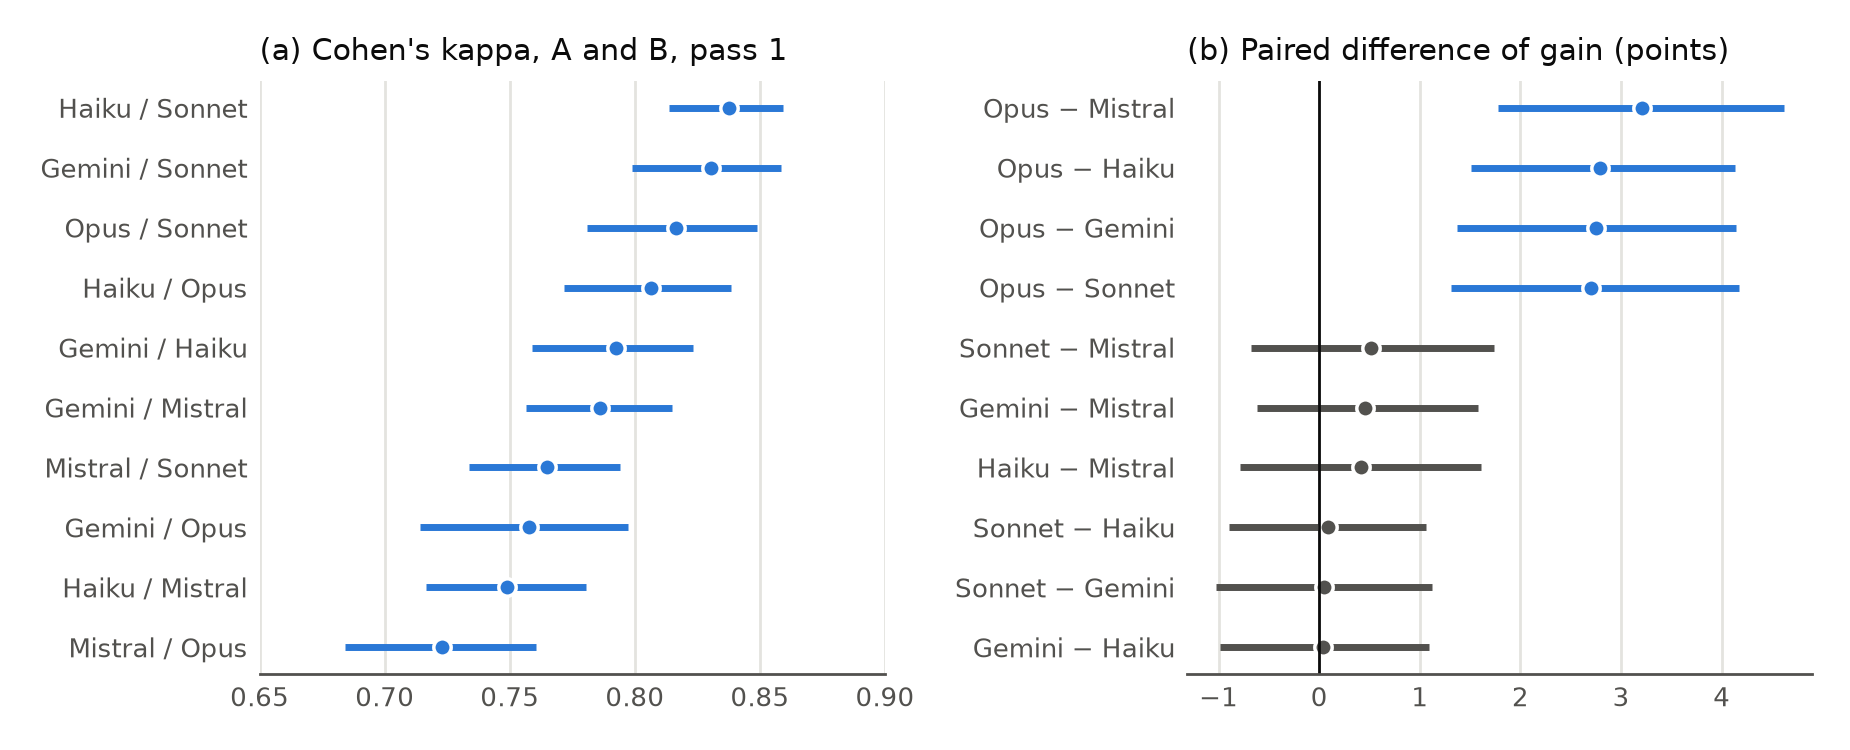
\includegraphics[width=0.8\linewidth]{fig_report_main.png}
\caption{The two central measures, with 95\% bootstrap intervals over features. (a)
Cohen's kappa of each pair of scorers, explanations A and B, pass 1, about 7,900 texts
per pair. (b) The 10 paired differences of gain over the placebo, each oriented as larger
minus smaller, in blue when the interval excludes 0. Gains per scorer are in
Table~\ref{tab:profile}.}
\label{fig:main}
\end{figure}

\subsection*{Judgments}

The raw agreement goes from 86.9\% (Mistral and Opus) to 92.6\% (Haiku and Sonnet), and
Cohen's kappa from 0.72 to 0.84, with intervals that do not overlap for the extreme pairs
(Figure~\ref{fig:main}a). Each scorer changes its own answer between two passes on only
0.1 to 3.1\% of the texts, so these disagreements are not sampling noise.

\subsection*{Gain}

The placebo works as a control: every scorer falls to chance, with 48.6 to 49.5\% of
right answers, so the texts carry no usable cue of their label\footnote{The values sit
slightly below 50\% because an unreadable answer counts as wrong.}. With the
explanations, the accuracy rises to 77 to 83\%, a gain of about 30 points for every
scorer (29.2 to 32.4, Table~\ref{tab:profile}).

Six of the ten paired differences lie between $-0.1$ and $+0.5$ points, with intervals of
about $\pm1.2$ points: Haiku, Sonnet, Gemini and Mistral draw a similar benefit from the
explanation, although no margin of equivalence was set in advance
(Figure~\ref{fig:main}b). The four others are those of Opus, which gains about 3 points
more than each of them (Opus minus Mistral: $+3.2$, [1.8, 4.6]). These four still exclude
0 when the ten intervals are corrected for multiple comparisons\footnote{Bonferroni
intervals, each at 99.5\%, so that the ten hold together at 95\%: Opus minus Mistral
[1.2, 5.2]. A robustness check added after the results (DEVIATIONS.md, entry 3).}.

\begin{table}[h]
\centering
\footnotesize
\begin{tabular}{lrrrrrrrrr}
\toprule
& Gain & \multicolumn{3}{c}{Sensitivity (\%)} & \multicolumn{3}{c}{Specificity (\%)} & Invalid & Changed \\
\cmidrule(lr){3-5}\cmidrule(lr){6-8}
Scorer & (pts) & A & B & placebo & A & B & placebo & (\%) & (\%) \\
\midrule
Haiku 5.5 & 29.6 & 62.1 & 67.1 & 1.5 & 92.2 & 91.5 & 95.9 & 1.2 & 3.1 \\
Sonnet 5.5 & 29.7 & 60.3 & 67.4 & 1.1 & 94.9 & 94.2 & 98.0 & 0.2 & 1.4 \\
Opus 5.5 & 32.4 & 71.2 & 75.0 & 2.1 & 90.1 & 90.0 & 96.2 & 0.9 & 2.3 \\
Gemini 2.5 Flash & 29.6 & 58.7 & 65.6 & 1.2 & 95.7 & 96.2 & 97.6 & 0.2 & 0.2 \\
Mistral Small 3.2 & 29.2 & 60.9 & 63.6 & 1.2 & 93.6 & 94.6 & 96.8 & 0.6 & 0.1 \\
\bottomrule
\end{tabular}
\caption{Profile per scorer, mean of both passes. Gain: accuracy with A and B minus
accuracy with the placebo. Sensitivity: positives answered 1. Specificity: negatives
answered 0. Invalid: unreadable answers after one retry. Changed: texts answered
differently by the two passes.}
\label{tab:profile}
\end{table}

\subsection*{Where the differences come from}

With as many positives as negatives, the gain splits into two parts:
\[
\text{gain} = \tfrac12\,(\text{sens}_{AB}-\text{sens}_P) + \tfrac12\,(\text{spec}_{AB}-\text{spec}_P).
\]
For every scorer, the first part makes the gain (30.5 to 35.5 points), and the second is
a small loss (0.8 to 3.1 points). In other words, the explanation makes a scorer find many
more positives, and raise a few more false alarms (Table~\ref{tab:profile}).

Opus is the clearest case. It finds 73\% of the positives, against 62 to 65\% for the
others, and answers 1 to about 10\% of the negatives, against 4 to 7\%.

\textit{Interpretation.} Its larger
gain thus seems to come from a lower threshold for answering ``yes'', rather than from a
better reading of the explanation.

\subsection*{The texts where the scorers disagree}

The five scorers are not unanimous on 1,568 texts (20\%). I drew 30 of them, 15
positives and 15 negatives, and had two fresh LLM agents propose the cause of each
disagreement\footnote{The agents (Claude Fable 5.2) were blind to the names of the
scorers, but not to the labels and activations. I also read the 30 texts. My reading
broadly agrees with theirs, but I did not record it text by text.}. They agree on 25
of the 30 (kappa 0.79), and attribute 18 to 21 of them to the explanation or the text
rather than to an error of the scorer. For example, a feature explained as ``references
to radio'' fires on ``Radio'' in ``Radioactive Man'', and the lone scorer that answers 1
is right. These causes are hypotheses rather than measurements.

\subsection*{Do the scorers pick the same explanation?}

This analysis is exploratory, and was decided after the results (DEVIATIONS.md, entry 2).
Across the 200 explanations, the scorers rank the accuracies alike (Spearman 0.76 to
0.90). Choosing between A and B for a given feature is less stable: two scorers pick
opposite explanations on 13\% (Haiku and Sonnet, [7, 20]) to 27\% (Opus and Gemini, [18,
36]) of the features, while a scorer compared with itself, pass 1 against pass 2, does so
on 0 to 7\%. On 47 of the 100 features, at least two scorers prefer opposite
explanations. These preferences rest on 40 texts per feature.

\section{Conclusion}

I can thus conclude that, on this SAE and with this prompt, the five scorers draw
a similar average benefit from an explanation, within about 3 points, while two of them
disagree on about one text in ten. The placebo shows that the benefit is real, since every
scorer falls to chance without the explanation. The larger gain of Opus comes with more
false alarms, and much of the disagreement appears to come from explanations that do not
describe the feature exactly. Finally, the scorers rank explanations alike overall, but
on almost half of the features at least two of them would retain a different one of the
two explanations.

The next step is to score new texts for the same explanations, comparing one scorer on
two disjoint sets of texts with two scorers on the same set, to tell whether these
reversals come from the scorer or from the choice of the texts.

\subsection*{What this does not show}

High agreement is not validity: scorers can be wrong together. A gain shows that the
explanation helps to predict activations, not that it describes a mechanism.

The study covers one SAE, one layer, 100 features and one prompt, with five scorers of
which three are Claude models. The settings differ by scorer, so a difference between
two scorers mixes the model and its setting. The positives come from stored examples,
not from the natural distribution, and nothing reliable can be said about A against B
for a given feature.

\subsection*{Prior work and AI assistance}

Setup, prompt, feature draw, placebos and code were prepared before the kick-off (20
November, 18:00), and every scorer call and analysis was made on 21 November. This report
and the code were generated with Claude (Claude Opus 5.5). I checked them and made every
design decision.

\subsection*{References}

{\footnotesize
\bibentree{Chen, X. (2026). Scoring explanations without reading them: structural
shortcuts in automated-interpretability evaluation data. arXiv:2610.37676.}
\bibentree{Paulo, G., Mallen, A., Juang, C., \& Belrose, N. (2024). Automatically
interpreting millions of features in large language models. arXiv:2410.13928.}
\bibentree{Van der Ben, S., Roch, N., Hedstr\"om, A., \& El-Assady, M. (2026). Building
fast, evaluating slow: pipeline choices dominate autointerpretability score variance.
arXiv:2607.19386.}
}

\end{document}
